% Permission is granted to copy, distribute and/or modify this document
% under the terms of the GNU Free Documentation License, Version 1.3
% or any later version published by the Free Software Foundation;
% with no Invariant Sections, no Front-Cover Texts, and no Back-Cover Texts.
% A copy of the license is included in the section entitled "GNU
% Free Documentation License".
%
% Written (C) 2012-2013 Heiko Strathmann

\section{Two-Sample-Testing with the Maximum Mean Discrepancy}
\label{sec:mmd_into}
An important class of hypothesis tests are the \emph{two-sample tests}, which will be defined in the following.
In two-sample testing, one tries to find out whether to sets of samples come from different distributions. Given two probability distributions $p,q$ and i.i.d.\ samples $X=\{x_i\}_{i=1}^m\subseteq \mathbb{R}^d\sim p$ and $Y=\{y_i\}_{i=1}^n\subseteq \mathbb{R}^d\sim p$, the two sample test distinguishes the hypothesises
\begin{align*}
H_0: p=q\\
H_A: p\neq q
\end{align*}

In order to solve this problem, it is desirable to have a criterion than takes a positive unique value if $p\neq q$, and zero if and only if $p=q$. The so called \emph{Maximum Mean Discrepancy} (MMD), has this property and allows to distinguish any two probability distributions, if used in a \emph{reproducing kernel Hilbert space} (RKHS). It is the distance of the mean embeddings $\mu_p, \mu_q$ of the distributions $p,q$ in such a RKHS $\mathcal{F}$ -- which can also be expressed in terms of expectation of kernel functions, i.e.
\begin{align}
\label{eqn:mmd_population}
\mmd[\mathcal{F},p,q]&=||\mu_p-\mu_q||_\mathcal{F}^2\\
&=\textbf{E}_{x,x'}\left[ k(x,x')\right]-
  2\textbf{E}_{x,y}\left[ k(x,y)\right]
  +\textbf{E}_{y,y'}\left[ k(y,y')\right]\notag
\end{align}
See \citep[Section 2]{Gretton2012} for details. We here only describe how to
use the MMD for two-sample testing. \shogun{} offers two types of test statistic based on the MMD, one with quadratic costs both in time and space, and on with linear time and constant space costs. Both come in different versions and with different methods how to approximate the null-distribution in order to construct a two-sample test.

\subsection{Quadratic Time MMD Statistic}
\label{sec:mmd_quadratic}
We now describe the quadratic time MMD, as described in \citep[Lemma
6]{Gretton2012}, which is implemented in \shogun{}. All methods in this section are implemented in \shogunclass{CQuadraticTimeMMD}, which accepts any type of \shogun{} features.

An unbiased estimate for expression \ref{eqn:mmd_population} can be obtained by estimating expected values with sample means
\begin{align*}
\mmd_u^2[\mathcal{F},X,Y]=&\frac{1}{m(m-1)}\sum_{i=1}^m\sum_{j\neq i}^mk(x_i,x_j) + \frac{1}{n(n-1)}\sum_{i=1}^n\sum_{j\neq i}^nk(y_i,y_j)\\
&-\frac{2}{mn}\sum_{i=1}^m\sum_{j\neq i}^nk(x_i,y_j)
\end{align*}

A biased estimate would be
\begin{align*}
\mmd_b^2[\mathcal{F},X,Y]=&\frac{1}{m^2}\sum_{i=1}^m\sum_{j=1}^mk(x_i,x_j) + \frac{1}{n^ 2}\sum_{i=1}^n\sum_{j=1}^nk(y_i,y_j)\\
&-\frac{2}{mn}\sum_{i=1}^m\sum_{j\neq i}^nk(x_i,y_j)
\end{align*}

To compute statistic, use \texttt{compute\_statistic}. To decide which statistic to use, use \texttt{set\_statistic\_type} with arguments \texttt{BIASED} or \texttt{UNBIASED} to activate this statistic type. Note that some methods for approximating the null-distribution only work with one of both types. Both statistics' computational costs are quadratic both in time and space. Note that the method returns $m\mmd_b^2[\mathcal{F},X,Y]$ since null distribution approximations work on $m$ times null distribution.

\subsubsection{Bootstrapping}
As for any two-sample test in \shogun{}, bootstrapping can be used to approximate the null-distribution with both types of quadratic MMD statistic. This results in a consistent, but slow test. Note that for each sample, the quadratic time estimate has to be re-computed. The number of samples to take is the only parameter. If unsure what to do, bootstrapping is the recommended way of constructing a test. As a rule of thumb, use at least 250 samples.
See \texttt{bootstrap\_null} in \shogunclass{CTwoDistributionsTestStatistic} and \shogunclass{CKernelTwoSampleTestStatistic}. Strongly consider using pre-computed kernel matrices as described in section \ref{sec:quadratic_mmd_precomputed_kernel}.

\subsubsection{Spectrum Approximation}
Approximates the null-distribution using the Eigen-Spectrum of the kernel matrix of the joint samples. Was described in \citep{Gretton2012b}. This is a fast and consistent test. Effectively, the null-distribution of the biased statistic is sampled, but in a more efficient way than the bootstrapping approach. The converges as

\begin{align}
\label{eqn:quadratic_mmd_spectrum}
m\mmd^2_b \rightarrow \sum_{l=1}^\infty \lambda_l z_l^2
\end{align}
where $z_l\sim \mathcal{N}(0,2)$ are i.i.d. normal samples and $\lambda_l$
Eigenvalues of expression 2 in \citep{Gretton2012b}, which can be empirically
estimated by $\hat\lambda_l=\frac{1}{m}\nu_l$ where $\nu_l$ are the Eigenvalues
of the centred kernel matrix of the joint samples $X$ and $Y$. The distribution
in expression \ref{eqn:quadratic_mmd_spectrum} can be easily sampled. \shogun{}'s implementation has two parameters:
\begin{itemize}
\item Number of samples from null-distribution. The more, the more accurate. As a rule of thumb, use 250.
\item Number of Eigenvalues of the Eigen-decomposition of the kernel matrix to use. The more, the better the results get; however, the Eigen-spectrum of the joint gram matrix usually decreases very fast. See \citep{Gretton2012b} for details.
\end{itemize}
If the kernel matrices are diagonal dominant, this method is likely to fail. For that and more details, see the original paper. Computational costs are much lower than bootstrapping, which is the only consistent alternative. Since Eigenvalues of the gram matrix has to be computed, costs are in $\mathcal{O}(m^3)$.

To get a number of samples, use \texttt{sample\_null\_spectrum}; to use that method for testing, use \texttt{set\_null\_approximation\_method(MMD2\_SPECTRUM)}. Both methods are to be found in \shogunclass{CQuadraticTimeMMD}. \textbf{Important:} This method only works with the biased statistic.

\subsubsection{Gamma Approximation}
\todo{Gamma Approximation: Merge with compute statistic in code and document! H.S.}
Another method for approximating the null-distribution is by matching the first two moments of a gamma-distribution and then use that. This is not consistent, but usually also gives good results while being very fast. However, there are distributions where the method fails; therefore, the type I error should always be monitored. Described in \citep{Gretton2012b}. It uses
\begin{align}
\label{eqn:quadratic_mmd_gamma}
m\mmd_b(Z) \sim \frac{x^{\alpha-1}\exp(-\frac{x}{\beta})}{\beta^\alpha \Gamma(\alpha)}
\end{align}
where
\begin{align*}
\alpha=\frac{(\textbf{E}(\text{MMD}_b(Z)))^2}{\var(\text{MMD}_b(Z))} \qquad \text{and} \qquad
 \beta=\frac{m \var(\text{MMD}_b(Z))}{(\textbf{E}(\text{MMD}_b(Z)))^2}
\end{align*}

Then, any threshold and p-value can be computed using the gamma distribution in expression \ref{eqn:quadratic_mmd_gamma}. Computational costs are in $\mathcal{O}(m^2)$.

To use that method for testing, use \texttt{set\_null\_approximation\_method(MMD2\_GAMMA)}, to be found in \shogunclass{CQuadraticTimeMMD}. \textbf{Important:} This method only works with the biased statistic.


\subsection{Linear Time MMD Statistic}
\label{sec:mmd_linear}
We now describe the linear time MMD, as described in \citep[Section
6]{Gretton2012}, which is implemented in \shogun{}. All methods in this section are implemented in \shogunclass{CLinearTimeMMD}.

A fast, unbiased estimate for expression \ref{eqn:mmd_population} which still uses all available data can be obtained by dividing data into two parts and then compute

\begin{align*}
\mmd_l^2[\mathcal{F},X,Y]=\frac{1}{m_2}\sum_{i=1}^{m_2} k(x_{2i},x_{2i+1})+k(y_{2i},y_{2i+1})-k(x_{2i},y_{2i+1})-
  k(x_{2i+1},y_{2i})
\end{align*}
where $ m_2=\lfloor\frac{m}{2} \rfloor$. While the above expression assumes that $m$ data are available from each distribution, the statistic in general works in an online setting where features are obtained one by one. Since only pairs of four points are considered at once, this allows to compute it on data streams. In addition, the computational costs are linear in the number of samples that are considered from each distribution. These two properties make the linear time MMD very applicable for large scale two-sample tests. In theory, any number of samples can be processed -- time is the only limiting factor.

\subsubsection*{How to Pass Data to \shogunclass{CLinearTimeMMD}}
To account for this streaming nature of the linear time MMD, the implementation in \shogun{} is based on the streaming framework around the class \shogunclass{CStreamingFeatures}. The latter basically implements an interface to get data one by one or in larger blocks. See section \ref{sec:shogun_objects-features-streaming} for more details on the streaming interface. If \shogunclass{CLinearTimeMMD} should be used on non-streaming data, such as for example \shogunclass{CDenseFeatures} as described in section \ref{sec:shogun_objects-features-dense}, simply construct an instance of \shogunclass{CStreamingFeatures} from these. For example, \shogunclass{CStreamingDenseFeatures} offers a constructor to construct an instance from an object of type \shogunclass{CDenseFeatures} which then can be passed to  \shogunclass{CLinearTimeMMD}. If a streaming feature class for your desired data does not exist or does not offer an constructor to build from an object in memory, write to the mailing list.
\textbf{Important:} The underlying parser of \shogunclass{CDenseFeatures} has to be started (or ensured that it is not needed) before \shogunclass{CLinearTimeMMD} computes anything. Otherwise, a deadlock might occur.

After streaming data is passed to \shogunclass{CLinearTimeMMD}, all interfaces work as before -- with the difference that new data is taken from the stream in every call of \texttt{compute\_statistic} and related methods. Note that taking data from the stream one by one results in a very inefficient way of computing the statistic due to involved overhead in the framework. To avoid this, there is an optional constructor parameter to specify a blocksize (note there is a default value). This number specifies how many samples are taken from the stream at once. The statistic then is computed in bursts on these blocks. In principle, the blocksize should be as large as possible, however, the memory consumption increases linear in the number of samples per block.
If set larger than $m$, all samples will be processed at once.

\subsubsection{Bootstrapping}
As for any two-sample test in \shogun{}, bootstrapping can be used to approximate the null distribution. This results in a consistent, but slow test. The number of samples to take is the only parameter. As a rule of thumb, use at least 250 samples.
See \texttt{bootstrap\_null} in \shogunclass{CLinearTimeMMD}.
Note that since \shogunclass{CLinearTimeMMD} operates on streaming features, \emph{new} data is taken from the stream in every iteration. This is in contrast to the usual way of bootstrapping as described in algorithm \ref{alg:bootstrapping}, where data is permuted in every iteration.

Also note that in general, bootstrapping is not really necessary since with the Gaussian approximation, a fast and consistent estimate of the null-distribution is available for the linear time MMD. However, to ensure that the Gaussian approximation is accurate, it should always be checked against bootstrapping at least once.

\subsubsection{Gaussian Approximation}
Since both the null- and the alternative distribution are Gaussian with equal variance (and different mean), it is possible to approximate the null-distribution by using a linear time estimate for this variance. An unbiased, linear time estimator for
\begin{align*}
\var[\mmd_l^2[\mathcal{F},X,Y]]
\end{align*}
can simply be computed by computing the empirical variance of
\begin{align*}
k(x_{2i},x_{2i+1})+k(y_{2i},y_{2i+1})-k(x_{2i},y_{2i+1})-k(x_{2i+1},y_{2i}) \qquad (1\leq i\leq m_2)
\end{align*}
A normal distribution with this variance and zero mean can then be used as an approximation for the null-distribution. This results in a consistent test and is very fast. However, note that it is an approximation and its accuracy depends on the underlying data distributions. It is a good idea to compare to the bootstrapping approach first to determine an appropriate number of samples to use. This number is usually in the tens of thousands.

To use the method for testing, use \texttt{set\_null\_approximation\_method(MMD1\_GAUSSIAN)}, to be found in \shogunclass{CLinearTimeMMD}. Using the Gaussian approximation, the null distribution can be estimated on the fly while computing the test statistic. The method \texttt{compute\_statistic\_and\_variance} does exactly this (results written into parameter references). The \texttt{perform\_test} methods of \shogunclass{CTestStatistic} for performing a complete two-sample are overwritten to make use of this more efficient approach. Use these instead of computing statistic and p-value separately.

\subsection{Precomputed Kernel Matrices for Quadratic Time MMD}
\label{sec:quadratic_mmd_precomputed_kernel}
For all MMD-based two-sample-tests, elements of kernel matrices of sample data have to be used. By default, all computations are done \emph{in-place} when possible, which means that the underlying kernel is evaluated on the fly (There are exceptions, when the matrix has to be stored, for example in order so solve Eigenvalue problems). However, for the quadratic time MMD, this may be inefficient when statistics are computed multiple times -- as in bootstrapping. Therefore, it is possible to initialize \shogunclass{CQuadraticTimeMMD} with a pre-computed \shogunclass{CCusotmKernel}. This kernel may be computed from any other kernel by simply passing the latter to the constructor of \shogunclass{CCusotmKernel}. This should be done whenever the kernel matrix fits into memory; it greatly improves performance. In bootstrapping, the kernel matrix only has to be permuted instead of being re-computed in every iteration. But there is also a (small) advantage for all other methods since \shogun{} computes kernel matrices in multiple threads.

In contrast, \shogunclass{CLinearTimeMMD} should not be used with \shogunclass{CCusotmKernel}s since it does not even need all elements -- so pointless computations would be made. Also, \shogunclass{CLinearTimeMMD} might be c

\subsection{Kernel Selection for MMD}
\label{sec:statistical_tests-mmd-kernel_selection}

\shogun{}'s kernel selection methods for MMD based two-sample tests are all based around  \cite{Sriperumbudur2009, Gretton2012a}. For the \shogunclass{CLinearTimeMMD}, \cite{Gretton2012a} describes a way of selecting the \emph{optimal} kernel in the sense that the test's type II error is minimised. For the linear time MMD, this is the method of choice. It is done via maximising the MMD statistic divided by its standard deviation and it is possible for single kernels and also for convex combinations of them. For the \shogunclass{CQuadraticTimeMMD}, the best method in literature is choosing the kernel that maximised the MMD statistic. For convex combinations of kernels, this can be achieved via a $L2$ norm constraint. A detailed comparison of all methods on numerous datasets can be found in \cite{Strathmann2012}.

MMD Kernel selection on \shogun{} always involves an implementation of the base class \shogunclass{CMMDKernelSelection}, which defines the interface for kernel selection. If combinations of kernel should be considered, there is a sub-class \shogunclass{CMMDKernelSelectionComb}. In addition, it involves setting up a number of baseline kernels $\mathcal{K}$ to choose from/combine in the form of a \shogunclass{CCombinedKernel}. All methods compute their results for a fixed set of these baseline kernels. We later give an example how to use these classes after providing a list of available methods.

\paragraph{\shogunclass{CMMDKernelSelectionMedian}:} Selects from a set \shogunclass{CGaussianKernel} instances the one whose width parameter is closest to the median of the pairwise distances in the data. The median is computed on a certain number of points from each distribution that can be specified as a parameter. Since the median is a stable statistic, one does not have to compute all pairwise distances but rather just a few thousands. This method a useful (and fast) heuristic that in many cases gives a good hint on where to start looking for Gaussian kernel widths. It is for example described in \citep{Gretton2012}. Note that it may fail badly in selecting a good kernel for certain problems.

\paragraph{\shogunclass{CMMDKernelSelectionMax}:} Selects from a set of arbitrary baseline kernels a single one that maximises the used MMD statistic -- more specific its estimate.
\begin{align*}
k^*=\argmax_{k\in\mathcal{K}} \hat \eta_k,
\end{align*}
where $\eta_k$ is an empirical MMD estimate for using a kernel $k$.
This was first described in \cite{Sriperumbudur2009} and was empirically shown to perform better than the median heuristic above. However, it remains a heuristic that comes with no guarantees. Since MMD estimates can be computed in linear and quadratic time, this method works for both methods. However, for the linear time statistic, there exists a better method.
 
\paragraph{\shogunclass{CMMDKernelSelectionOpt}:} Selects the optimal single kernel from a set of baseline kernels. This is done via maximising the ratio of the linear MMD statistic and its standard deviation.
\begin{align*}
k^*=\argmax_{k\in\mathcal{K}} \frac{\hat \eta_k}{\hat\sigma_k+\lambda},
\end{align*}
where $\eta_k$ is a linear time MMD estimate for using a kernel $k$ and $\hat\sigma_k$ is a linear time variance estimate of $\eta_k$ to which a small number $\lambda$ is added to prevent division by zero.
These are estimated in a linear time way with the streaming framework that was described in section \ref{sec:mmd_linear}. Therefore, this method is only available for \shogunclass{CLinearTimeMMD}. Optimal here means that the resulting test's type II error is minimised for a fixed type I error. \emph{Important:} For this method to work, the kernel needs to be selected on \emph{different} data than the test is performed on. Otherwise, the method will produce wrong results.
 
\paragraph{\shogunclass{CMMDKernelSelectionCombMaxL2}:} Selects a convex combination of kernels that maximises the MMD statistic. This is the multiple kernel analogous to \shogunclass{CMMDKernelSelectionMax}. This is done via solving the convex program
\begin{align*}
\boldsymbol{\beta}^*=\min_{\boldsymbol{\beta}} \{\boldsymbol{\beta}^T\boldsymbol{\beta}  :  \boldsymbol{\beta}^T\boldsymbol{\eta}=\mathbf{1}, \boldsymbol{\beta}\succeq 0\},
\end{align*}
where $\boldsymbol{\beta}$ is a vector of the resulting kernel weights and $\boldsymbol{\eta}$ is a vector of which each component contains a MMD estimate for a baseline kernel. See \citep{Gretton2012a} for details. Note that this method is unable to select a single kernel -- even when this would be optimal.
Again, when using the linear time MMD, there are better methods available.

\paragraph{\shogunclass{CMMDKernelSelectionCombOpt}:} Selects a convex combination of kernels that maximises the MMD statistic divided by its covariance. This corresponds to \emph{optimal} kernel selection in the same sense as in class \shogunclass{CMMDKernelSelectionOpt} and is its multiple kernel analogous. The convex program to solve is
\begin{align*}
\boldsymbol{\beta}^*=\min_{\boldsymbol{\beta}} (\hat Q+\lambda I) \{\boldsymbol{\beta}^T\boldsymbol{\beta}  :  \boldsymbol{\beta}^T\boldsymbol{\eta}=\mathbf{1}, \boldsymbol{\beta}\succeq 0\},
\end{align*}
where again $\boldsymbol{\beta}$ is a vector of the resulting kernel weights and $\boldsymbol{\eta}$ is a vector of which each component contains a MMD estimate for a baseline kernel. The matrix $\hat Q$ is a linear time estimate of the covariance matrix of the vector $\boldsymbol{\eta}$ to whose diagonal a small number $\lambda$ is added to prevent division by zero. See \citep{Gretton2012a} for details. In contrast to \shogunclass{CMMDKernelSelectionCombMaxL2}, this method is able to select a single kernel when this gives a lower type II error than a combination. In this sense, it contains \shogunclass{CMMDKernelSelectionOpt}.

\paragraph{Procedure}
In order to use one of the above methods for kernel selection, one has to create a new instance of \shogunclass{CCombinedKernel} and use the method \texttt{append\_kernel} to append all desired baseline kernels to it. This combined kernel is then passed to the MMD class. Then, an object of any of the above kernel selection methods is created and the MMD instance is passed to it in the constructor. There are then multiple methods to call
\begin{itemize}
\item \texttt{compute\_measures} returns a vector kernel selection criteria if a single kernel selection method is used. It will return a vector of selected kernel weights if a combined kernel selection method is used. For \shogunclass{CMMDKernelSelectionMedian}, the method does throw an error.

\item \texttt{select\_kernel} returns the selected kernel of the method. For single kernels this will be one of the baseline kernel instances. For the combined kernel case, this will be the underlying \shogunclass{CCombinedKernel} instance where the subkernel weights are set to the weights that were selected by the method. 
\end{itemize}

In order to utilise the selected kernel, it has to be passed to an MMD instance via \texttt{set\_kernel} or the constructor. See the examples for more details.

\subsubsection{Examples}
There are graphical python examples which plot example data, alternative and null-distributions. See figures \ref{fig:statistical_testing-quadratic_time_mmd} and \ref{fig:statistical_testing-linear_time_mmd} for a screenshot for quadratic and linear time MMD respectively. In addition there are examples for linear time and quadratic time MMD that illustrate how to estimate type I and type II errors rates, and how to use kernel selection methods.

\begin{figure}\centering
		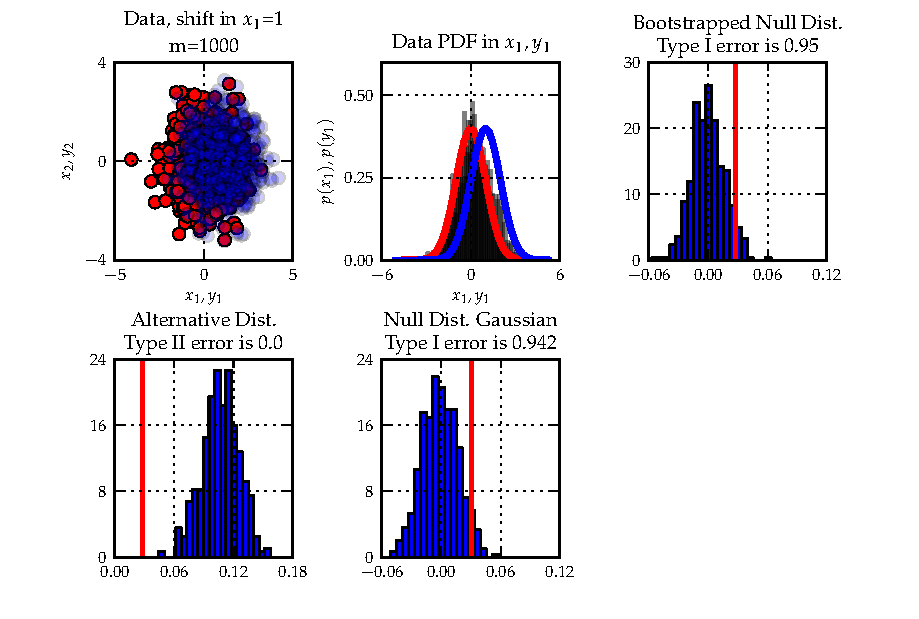
\includegraphics{fig/statistical_testing/linear_time_mmd}
		\caption{Screenshot of graphical python example for linear time MMD.}
		\label{fig:statistical_testing-linear_time_mmd}
\end{figure}

\begin{figure}\centering
		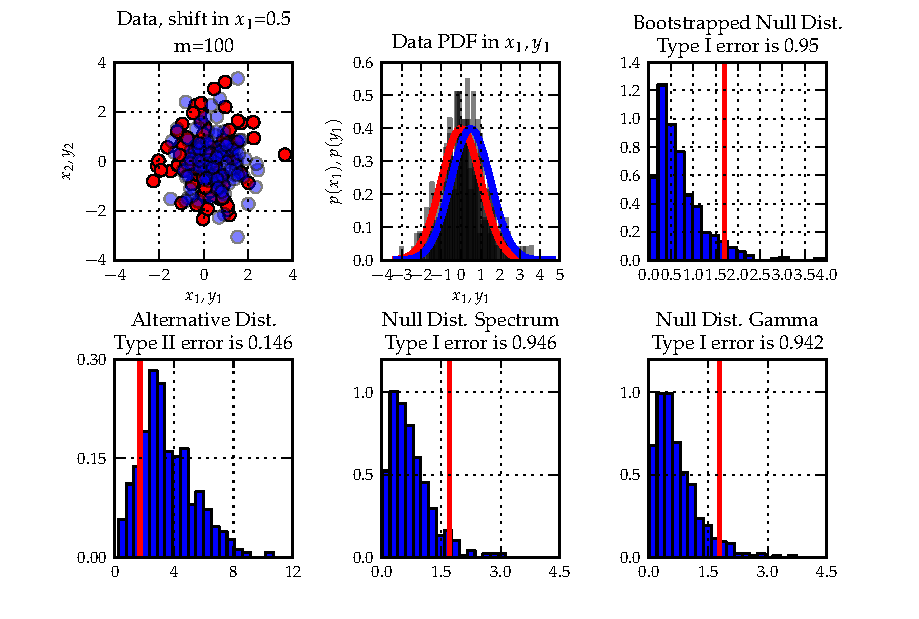
\includegraphics{fig/statistical_testing/quadratic_time_mmd}
		\caption{Screenshot of graphical python example for quadratic time MMD.}
		\label{fig:statistical_testing-quadratic_time_mmd}
\end{figure}